\documentclass{asaproc}

\usepackage{graphicx}
\usepackage{bm}
\newcommand{\m}[1]{\mathbf{\bm{#1}}}
\newcommand{\R}{I\hspace{-4.4pt}R}

%\usepackage{times}
%If you have times installed on your system, please
%uncomment the line above

%For figures and tables to stretch across two columns
%use \begin{figure*} \end{figure*} and
%\begin{table*}\end{table*}
% please place figures & tables as close as possible
% to text references


\newcommand{\be}{\begin{equation}}
\newcommand{\ee}{\end{equation}}

\title{Modeling Thefts in California Counties in 2010}

%input all authors' names

\author{Mickey Warner \\ AMS 207}

%input affiliations

%{USDA Forest Service Forest Products Laboratory}

\begin{document}

\maketitle


\begin{abstract}
For the year 2010, counts of four types of theft (robbery, burglary, larceny, and motor vehicle) were recorded for 39 counties in California. The log-transformation is applied to the counts and the log-counts are modeled hierarchically as a multivariate normal of dimension four. We show that the multivariate normal provides a reasonable fit to the log-counts and report a summary for the predictive distributions for each theft by county.
\end{abstract}

\section{Introduction}

The data set we analyze in this paper contains the number of thefts (either robbery, burglary, larceny, or motor vehicle) for 39 California counties in 2010. The population for each county is also given, though we do not use this information in the analysis. We would expect that as population increases, the number of thefts also increase. By plotting population against each theft (not shown), we see that the relationship between population and theft count may be reasonably modeled under a multivariate regression framework. However, even with a log-transformation, the regression approach would have difficulty handling the hetereoskedasticity that is present. We suspect there would also be issues in modeling those very low or very high population counties.

An alternative approach, the one we take in this paper, is to model the log theft counts hierarchically and to omit the population altogether. Figure \ref{data} presents scatter plots of the four theft types for the original data (left) and the log-transformed data (right). The log transformation seems to suggest that a multivariate normal model is suitable. It is true that higher population counties observed greater numbers of thefts, but the hierarchical setting allows us the flexibility to dealing with any peculiarities. For instance, Sacramento county had an unusually low number of motor vehicle thefts considering it ranked near the top in all other thefts and is one of the most populated counties. The hierarchical model would account for this, whereas we could run the risk of overfitting in the regression case.

In section 2 we describe the details of the model and the model fitting procedure. A posterior analysis is given in section 3. We conclude with a discussion in section 4.

\begin{figure*}[ht]
\centering
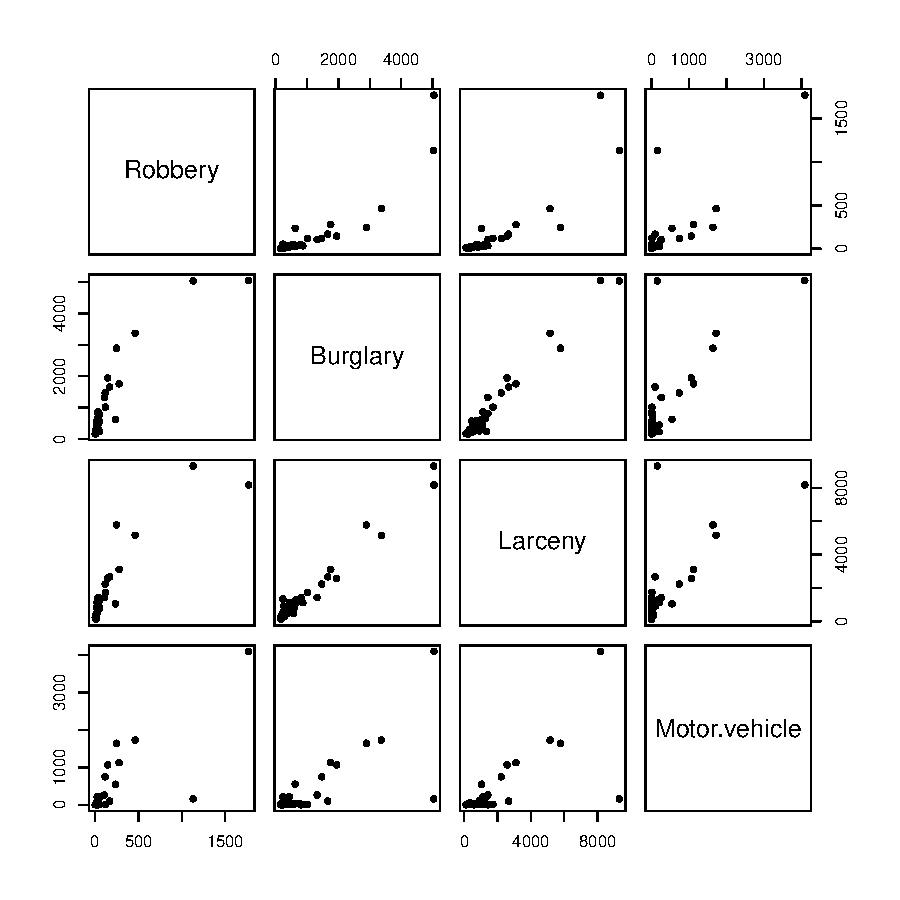
\includegraphics[scale=0.55]{figs/data.pdf}
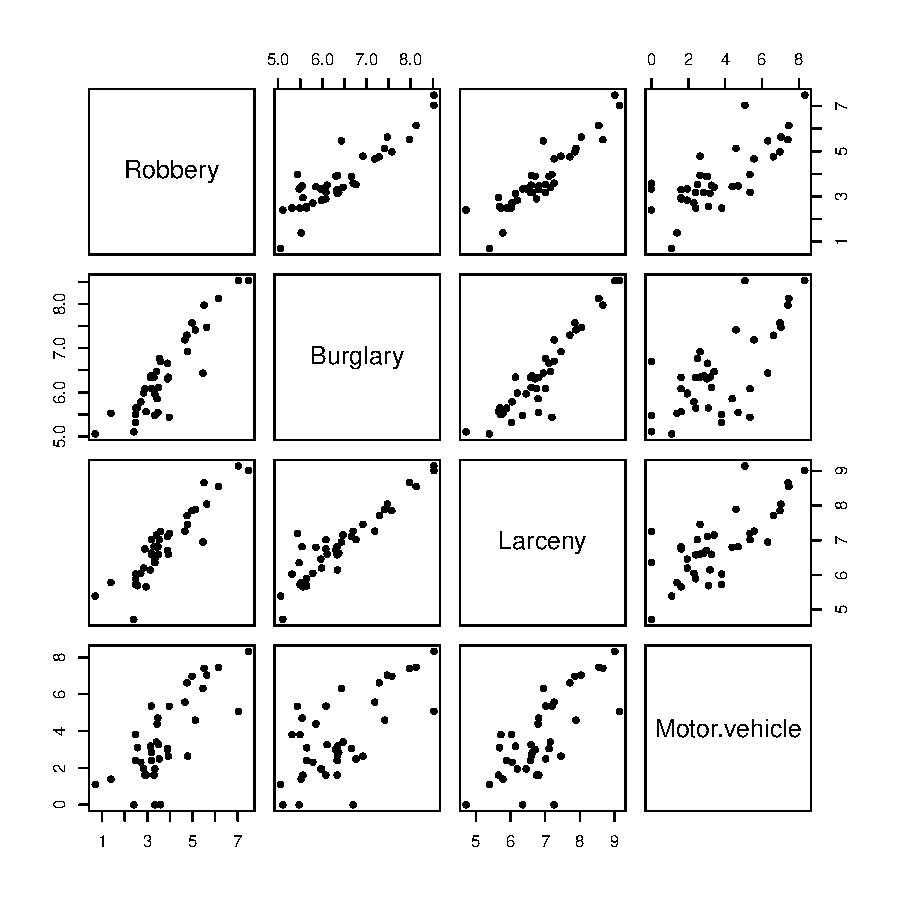
\includegraphics[scale=0.55]{figs/data_log.pdf}
\caption{Scatter plots for the number of thefts by county. The left set of plots is the original data while the right set is of the log-transformed data.}
\label{data}
\end{figure*}

\section{Methods}

\subsection{Hierarchical model}

Denote $\m{z}_i$ as the vector of length $p=4$ containing the log theft counts for county $i=1,\ldots,n=39$. We assume a normal likelihood for each $\m{z}_i$
\begin{eqnarray}
\m{z}_i|\m{\mu}_i,\Sigma &\sim& N(\m{\mu}_i, \Sigma)
\end{eqnarray}
and the following priors
\begin{eqnarray}
\m{\mu}_i|\m{\mu},V &\sim& N(\m{\mu}, V) \\
\m{\mu} &\sim& N(\m{m}, C_0) \\
\Sigma &\sim& IW(S_0, r) \\
V &\sim& IW(D_0, k).
\end{eqnarray}
The likelihood assumes that the observation from each county comes from its own normal population. The prior on $\m{\mu}_i$ (2) constrains the county means so we do not risk overfitting, which seems plausible given each observation has its own mean. We assume independence among $\m{\mu}$, $\Sigma$, and $V$ and that $\m{\mu}_i$ are all independent.

Other prior specifications may model the data better, but these choices (2)-(5) result in convenient full posterior conditionals which we discuss later. The constants $\m{m}$, $C_0$, $S_0$, $r$, $D_0$, and $k$ are chosen to be rather non-informative. With only $n=39$ data points, we can not be as non-informative as we would like. We chose $\m{m}=\bar{\m{z}}$, $C_0=I_p$, $S_0=0.25 I_p$, $r=6$, $D_0=3 I_p$, and $k=5$, where $I_p$ is the $p\times p$ identity matrix. This reflects our expectation that the variance associated with each observation, $\Sigma$, should be ``smaller'' than the variance for the county means, $V$. Though not ideal, these priors were chosen after trial and error: they resulted in decent predictions while remaining somewhat non-informative.

\subsection{Parameter estimation}

As mentioned earlier, the prior specification results in convenient full conditionals. These are given by
\begin{eqnarray}
\m{\mu}_i|\cdot &\sim& N((\Sigma^{-1}+V^{-1})^{-1}(\Sigma^{-1}\m{z}_i+V^{-1}\m{\mu}), \nonumber \\
&& ~~~~~ ~~~~~ (\Sigma^{-1}+V^{-1})^{-1}) \\
\m{\mu}|\cdot &\sim& N((nV^{-1}+C_0^{-1})^{-1}(nV^{-1}\bar{\m{\mu}}+C_0^{-1}\m{m}), \nonumber \\
&& ~~~~~ ~~~~~ (nV^{-1}+C_0^{-1})^{-1}) \\
\Sigma|\cdot &\sim& IW(S_0+\sum_{i=1}^n(\m{z}_i-\m{\mu}_i)(\m{z}_i-\m{\mu}_i)^\top, r+n) \\
V|\cdot &\sim& IW(D_0+\sum_{i=1}^n(\m{\mu}_i-\m{\mu})(\m{\mu}_i-\m{\mu})^\top, k+n)
\end{eqnarray}
where the dot $(\cdot)$ represents the data and all other variables and $\bar{\m{\mu}}=1/n\sum_{i=1}^n\m{\mu}_i$. We are thus able to explore the posterior using direct sampling. We iteratively draw samples from each full conditional based on the most recent samples of the other parameters.

\section{Results}

We obtain $10000$ posterior draws after burning in $2000$ draws. There did not appear to be any convergence or ``stickiness'' issues with the sampler as often happens when estimating several variances. Posterior means for $\m{\mu}$, $\Sigma$, and $V$ are as follows
\begin{eqnarray*}
\m{\mu}&=&(3.761, 6.404, 6.863, 3.607)^\top \\
\Sigma&=&\left(\begin{array}{rrrr}
 0.096 &  0.032 &  0.031 & -0.004 \\
 0.032 &  0.066 &  0.028 & -0.008 \\
 0.031 &  0.028 &  0.065 & -0.004 \\
-0.004 & -0.008 & -0.004 &  0.127
\end{array}\right)  \\
V&=&\left(\begin{array}{rrrr}
1.912 & 1.079 & 1.184 & 2.241 \\
1.079 & 0.856 & 0.774 & 1.330 \\
1.184 & 0.774 & 0.991 & 1.553 \\
2.241 & 1.330 & 1.553 & 4.603
\end{array}\right)
\end{eqnarray*}
The labels of each component in $\m{\mu}$ are Robbery, Burglary, Larceny, and Motor.Vehicle. The same order applies for the covariance matrices. Posterior means for each $\m{\mu}_i$ will not be presented, instead tables of predictions based on $\m{\mu}_i$ are given later. The overall mean $\m{\mu}$ corresponds very closely to the mean log thefts of the data (only off by a few thousandths in each component). As expected, the $\Sigma$ is ``smaller'' than $V$ as it has a smaller variance in each diagonal element.

Since we have a hierarchical model, there are various ways to obtain posterior predictions. For a particular county, we could use its county mean, $\m{\mu}_i$, to make predictions by drawing $\m{z}_i^*$ from a $N(\m{\mu}_i,\Sigma)$. For a new county, we would need to draw $\m{\mu}_i^*$ from a $N(\m{\mu}, V)$ and then draw $\m{z}_i^*$ from $N(\m{\mu}_i^*,\Sigma)$. The predictions we will look at are based on the posterior samples for $\m{\mu}_i$, for $i=1,\ldots,39$.

Predictive distributions are obtained for each of the 39 counties and for each type of theft. Figure \ref{fit} shows our predictions (on the log-scale) compared to the observations. Equal-tailed 95\% posterior predictive probability intervals are represented by the vertical lines and black dots represent the mean predictions. Each black dot and line pair is for a particular county. The plot suggests that our model provides a reasonable fit to the data: the mean predictions are all very close to the line $y=x$ and every interval crosses the line. There is a slight tendency to overestimate lower theft counts and underestimate higher theft counts, but not so much to be concerned with.

After drawing a $\m{z}_i^*$ from $N(\m{\mu}_i, \Sigma)$ using the posterior samples for $\m{\mu}_i$ and $\Sigma$ we exponentiate the draw to get back to the original scale $\m{y}_i^*=\exp(\m{z}_i^*)$. We can use these back-transformed values to make inferences based on the theft counts for each county. Tables 1 through 4 contain summaries of all of these posterior predictive distributions. As expected, our model can predict a county's theft count fairly well. However, this has its drawbacks which we will discuss in the next section.

\begin{figure}[ht]
\centering
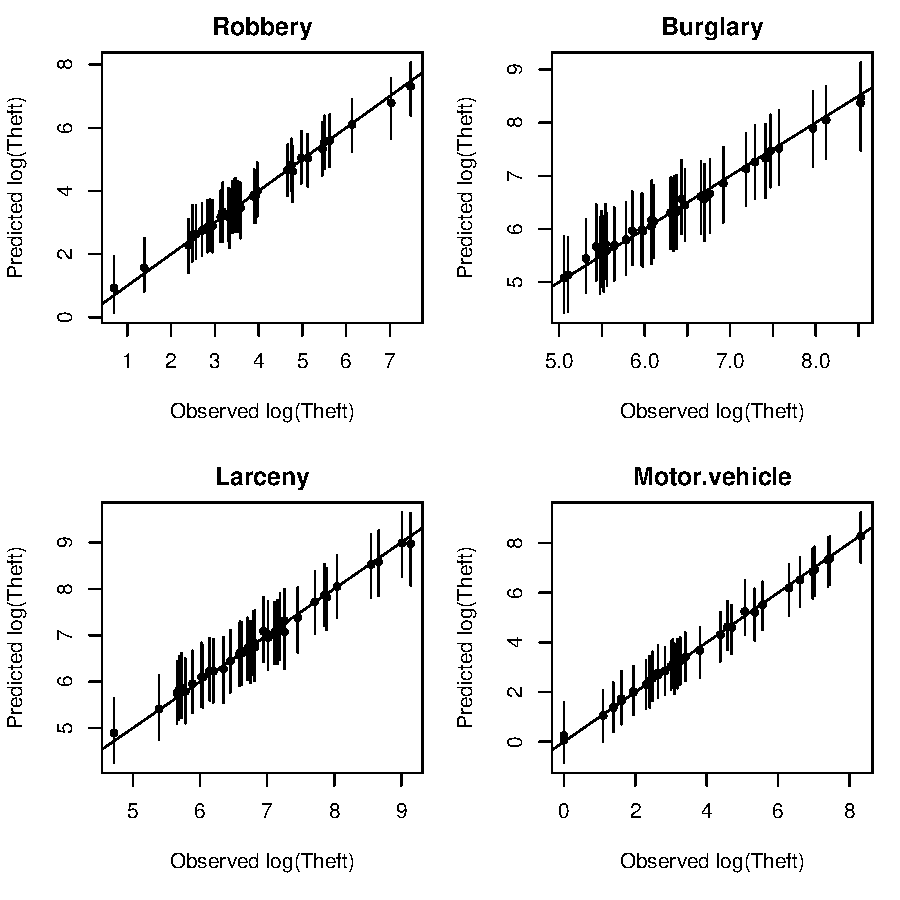
\includegraphics[scale=0.55]{figs/fit.pdf}
\caption{Plots of the posterior predictions (on the log-scale) against the observed log counts. The vertical lines represent equal-tailed 95\% probability intervals and the solid dots are the mean predictions. The diagonal line is the line $y=x$.}
\label{fit}
\end{figure}

Of particular interest is the probability of observing a total number of at least 3000 thefts in 2010 in Santa Cruz county. Santa Cruz county corresponds to observation $i=31$. Using the back-transformed posterior predictive draws $\m{y}_{31}^*$, of which we have 10000, we take each vector and add up its components $\sum_{j=1}^4 y_{31,j}^*$. The probability of observing more than 3000 total thefts in Santa Cruz is computed by counting how many of these vectors had a sum greater than 3000 and then dividing that number by 10000. Our model estimates this probability at $0.0605$.

\begin{table}[p!]
\caption{\enspace Summary of the predictive distributions for the number of robberies by county.}
\begin{tabular}{lrrrrr}
\\ [-5pt]
County & Obs & Mean & 2.5\% & 50\% & 97.5\% \\ 
  \hline
Alameda & 235 & 227 & 85 & 210 & 483 \\ 
  Butte & 24 & 27 & 11 & 25 & 54 \\ 
  Calaveras & 12 & 14 & 6 & 13 & 31 \\ 
  Contra Costa & 119 & 111 & 39 & 105 & 220 \\ 
  El Dorado & 34 & 37 & 14 & 34 & 76 \\ 
  Fresno & 116 & 135 & 55 & 123 & 290 \\ 
  Humboldt & 33 & 36 & 14 & 33 & 75 \\ 
  Imperial & 13 & 16 & 6 & 14 & 35 \\ 
  Kern & 463 & 483 & 186 & 453 & 971 \\ 
  Kings & 12 & 15 & 6 & 13 & 36 \\ 
  Lake & 17 & 19 & 8 & 17 & 40 \\ 
  Los Angeles & 1770 & 1645 & 585 & 1565 & 3221 \\ 
  Madera & 24 & 27 & 11 & 25 & 56 \\ 
  Marin County & 28 & 26 & 9 & 24 & 53 \\ 
  Mendocino & 19 & 20 & 8 & 18 & 41 \\ 
  Merced & 49 & 52 & 21 & 49 & 105 \\ 
  Monterey & 51 & 51 & 20 & 47 & 103 \\ 
  Napa & 2 & 3 & 1 & 2 & 7 \\ 
  Nevada & 4 & 5 & 2 & 5 & 12 \\ 
  Orange & 32 & 38 & 15 & 33 & 83 \\ 
  Placer & 30 & 35 & 14 & 32 & 74 \\ 
  Riverside & 247 & 286 & 115 & 262 & 588 \\ 
  Sacramento & 1131 & 988 & 293 & 951 & 1948 \\ 
  San Bernardino & 145 & 169 & 67 & 153 & 360 \\ 
  San Diego & 278 & 292 & 114 & 271 & 591 \\ 
  San Joaquin & 168 & 168 & 64 & 157 & 337 \\ 
  San Luis Obispo & 18 & 20 & 8 & 19 & 42 \\ 
  San Mateo & 53 & 60 & 24 & 53 & 133 \\ 
  Santa Barbara & 27 & 29 & 11 & 27 & 59 \\ 
  Santa Clara & 24 & 31 & 13 & 27 & 74 \\ 
  Santa Cruz & 36 & 35 & 12 & 33 & 72 \\ 
  Shasta & 23 & 26 & 11 & 24 & 56 \\ 
  Sonoma & 49 & 50 & 20 & 47 & 102 \\ 
  Stanislaus & 106 & 115 & 47 & 106 & 237 \\ 
  Sutter & 12 & 15 & 6 & 13 & 35 \\ 
  Tehama & 11 & 11 & 4 & 10 & 23 \\ 
  Tuolumne & 15 & 17 & 7 & 15 & 36 \\ 
  Ventura & 31 & 36 & 15 & 32 & 80 \\ 
  Yuba & 28 & 29 & 11 & 27 & 59 \\ 
   \hline
\end{tabular}
\end{table}

\begin{table}[p!]
\caption{\enspace Summary of the predictive distributions for the number of burglaries by county.}
\centering
\begin{tabular}{lrrrrr}
\\ [-5pt]
County & Obs & Mean & 2.5\% & 50\% & 97.5\% \\ 
  \hline
Alameda & 622 & 755 & 363 & 697 & 1498 \\ 
  Butte & 564 & 568 & 263 & 542 & 1029 \\ 
  Calaveras & 282 & 309 & 149 & 289 & 586 \\ 
  Contra Costa & 1011 & 1014 & 452 & 966 & 1850 \\ 
  El Dorado & 864 & 829 & 374 & 789 & 1505 \\ 
  Fresno & 1466 & 1515 & 728 & 1430 & 2817 \\ 
  Humboldt & 450 & 489 & 235 & 462 & 912 \\ 
  Imperial & 283 & 316 & 154 & 292 & 620 \\ 
  Kern & 3368 & 3285 & 1514 & 3139 & 5917 \\ 
  Kings & 243 & 283 & 136 & 261 & 573 \\ 
  Lake & 396 & 411 & 195 & 388 & 780 \\ 
  Los Angeles & 5046 & 5056 & 2225 & 4822 & 9165 \\ 
  Madera & 585 & 591 & 281 & 562 & 1078 \\ 
  Marin County & 239 & 266 & 120 & 251 & 508 \\ 
  Mendocino & 260 & 287 & 136 & 267 & 553 \\ 
  Merced & 778 & 787 & 369 & 748 & 1436 \\ 
  Monterey & 567 & 594 & 278 & 565 & 1082 \\ 
  Napa & 157 & 171 & 83 & 157 & 343 \\ 
  Nevada & 250 & 263 & 123 & 245 & 505 \\ 
  Orange & 255 & 325 & 160 & 296 & 660 \\ 
  Placer & 645 & 665 & 315 & 632 & 1232 \\ 
  Riverside & 2892 & 2850 & 1316 & 2706 & 5219 \\ 
  Sacramento & 5038 & 4624 & 1802 & 4472 & 8331 \\ 
  San Bernardino & 1942 & 1959 & 919 & 1846 & 3596 \\ 
  San Diego & 1755 & 1842 & 888 & 1744 & 3356 \\ 
  San Joaquin & 1656 & 1618 & 729 & 1553 & 2913 \\ 
  San Luis Obispo & 437 & 454 & 208 & 428 & 845 \\ 
  San Mateo & 229 & 314 & 152 & 284 & 640 \\ 
  Santa Barbara & 564 & 568 & 259 & 539 & 1039 \\ 
  Santa Clara & 438 & 512 & 248 & 471 & 1034 \\ 
  Santa Cruz & 812 & 756 & 306 & 725 & 1391 \\ 
  Shasta & 568 & 575 & 272 & 542 & 1074 \\ 
  Sonoma & 547 & 583 & 280 & 551 & 1088 \\ 
  Stanislaus & 1320 & 1327 & 631 & 1254 & 2470 \\ 
  Sutter & 203 & 248 & 122 & 227 & 504 \\ 
  Tehama & 165 & 181 & 86 & 168 & 352 \\ 
  Tuolumne & 325 & 350 & 169 & 329 & 666 \\ 
  Ventura & 349 & 415 & 207 & 383 & 812 \\ 
  Yuba & 390 & 419 & 200 & 395 & 785 \\ 
   \hline
\end{tabular}
\end{table}




\begin{table}[p!]
\caption{\enspace Summary of the predictive distributions for the number of larceny cases by county.}
\centering
\begin{tabular}{lrrrrr}
\\ [-5pt]
County & Obs & Mean & 2.5\% & 50\% & 97.5\% \\ 
  \hline
Alameda & 1041 & 1278 & 622 & 1184 & 2478 \\ 
  Butte & 721 & 755 & 357 & 720 & 1371 \\ 
  Calaveras & 361 & 407 & 198 & 378 & 778 \\ 
  Contra Costa & 1729 & 1686 & 754 & 1612 & 3072 \\ 
  El Dorado & 1114 & 1101 & 508 & 1053 & 1975 \\ 
  Fresno & 2230 & 2383 & 1165 & 2243 & 4425 \\ 
  Humboldt & 732 & 789 & 385 & 742 & 1465 \\ 
  Imperial & 295 & 357 & 177 & 330 & 710 \\ 
  Kern & 5152 & 5282 & 2513 & 5043 & 9580 \\ 
  Kings & 306 & 375 & 180 & 343 & 743 \\ 
  Lake & 492 & 532 & 254 & 502 & 987 \\ 
  Los Angeles & 8174 & 8467 & 3731 & 8074 & 15764 \\ 
  Madera & 755 & 792 & 386 & 751 & 1450 \\ 
  Marin County & 573 & 562 & 249 & 537 & 1030 \\ 
  Mendocino & 286 & 334 & 163 & 312 & 629 \\ 
  Merced & 1227 & 1234 & 577 & 1173 & 2249 \\ 
  Monterey & 735 & 793 & 381 & 753 & 1445 \\ 
  Napa & 219 & 239 & 116 & 222 & 472 \\ 
  Nevada & 324 & 349 & 167 & 326 & 673 \\ 
  Orange & 910 & 978 & 474 & 904 & 1896 \\ 
  Placer & 1275 & 1259 & 588 & 1187 & 2311 \\ 
  Riverside & 5776 & 5617 & 2627 & 5365 & 10236 \\ 
  Sacramento & 9309 & 8430 & 3360 & 8194 & 15004 \\ 
  San Bernardino & 2574 & 2773 & 1331 & 2615 & 5246 \\ 
  San Diego & 3106 & 3294 & 1563 & 3118 & 6090 \\ 
  San Joaquin & 2664 & 2624 & 1232 & 2516 & 4671 \\ 
  San Luis Obispo & 853 & 828 & 384 & 787 & 1516 \\ 
  San Mateo & 1332 & 1388 & 664 & 1290 & 2637 \\ 
  Santa Barbara & 912 & 897 & 421 & 858 & 1636 \\ 
  Santa Clara & 1113 & 1185 & 575 & 1103 & 2278 \\ 
  Santa Cruz & 1419 & 1258 & 526 & 1211 & 2294 \\ 
  Shasta & 466 & 541 & 263 & 506 & 1044 \\ 
  Sonoma & 821 & 874 & 423 & 829 & 1595 \\
  Stanislaus & 1421 & 1585 & 759 & 1492 & 2949 \\ 
  Sutter & 413 & 474 & 229 & 435 & 945 \\ 
  Tehama & 112 & 143 & 70 & 132 & 289 \\ 
  Tuolumne & 422 & 472 & 230 & 440 & 901 \\ 
  Ventura & 894 & 960 & 463 & 900 & 1809 \\ 
  Yuba & 634 & 665 & 318 & 630 & 1220 \\ 
   \hline
\end{tabular}
\end{table}

\begin{table}[p!]
\caption{\enspace Summary of the predictive distributions for the number of motor vehicle thefts by county.}
\centering
\begin{tabular}{lrrrrr}
\\ [-5pt]
County & Obs & Mean & 2.5\% & 50\% & 97.5\% \\ 
  \hline
Alameda & 549 & 557 & 162 & 505 & 1283 \\ 
  Butte & 11 & 13 & 5 & 11 & 31 \\ 
  Calaveras & 11 & 12 & 4 & 11 & 28 \\ 
  Contra Costa & 14 & 19 & 6 & 16 & 50 \\ 
  El Dorado & 12 & 15 & 5 & 13 & 36 \\ 
  Fresno & 746 & 750 & 229 & 693 & 1623 \\ 
  Humboldt & 26 & 29 & 10 & 26 & 67 \\ 
  Imperial & 22 & 23 & 7 & 21 & 53 \\ 
  Kern & 1726 & 1825 & 576 & 1659 & 4040 \\ 
  Kings & 45 & 45 & 13 & 41 & 99 \\ 
  Lake & 7 & 8 & 3 & 7 & 19 \\ 
  Los Angeles & 4090 & 4494 & 1412 & 4008 & 10277 \\ 
  Madera & 17 & 20 & 7 & 17 & 47 \\ 
  Marin County & 1 & 1 & 0 & 1 & 4 \\ 
  Mendocino & 5 & 6 & 2 & 5 & 14 \\ 
  Merced & 21 & 25 & 9 & 22 & 62 \\ 
  Monterey & 14 & 17 & 6 & 15 & 42 \\ 
  Napa & 3 & 3 & 1 & 3 & 8 \\ 
  Nevada & 4 & 4 & 2 & 4 & 11 \\ 
  Orange & 110 & 112 & 34 & 102 & 252 \\ 
  Placer & 30 & 34 & 11 & 30 & 80 \\ 
  Riverside & 1642 & 1683 & 511 & 1541 & 3793 \\ 
  Sacramento & 159 & 225 & 75 & 179 & 647 \\ 
  San Bernardino & 1064 & 1054 & 318 & 974 & 2263 \\ 
  San Diego & 1124 & 1163 & 363 & 1065 & 2573 \\ 
  San Joaquin & 98 & 116 & 40 & 101 & 286 \\ 
  San Luis Obispo & 5 & 6 & 2 & 5 & 15 \\ 
  San Mateo & 209 & 210 & 59 & 192 & 466 \\ 
  Santa Barbara & 5 & 6 & 2 & 5 & 17 \\ 
  Santa Clara & 211 & 208 & 58 & 190 & 461 \\ 
  Santa Cruz & 1 & 2 & 1 & 1 & 5 \\ 
  Shasta & 24 & 26 & 9 & 24 & 62 \\ 
  Sonoma & 20 & 23 & 8 & 21 & 55 \\ 
  Stanislaus & 261 & 277 & 93 & 251 & 620 \\ 
  Sutter & 45 & 45 & 13 & 41 & 97 \\ 
  Tehama & 1 & 1 & 0 & 1 & 3 \\ 
  Tuolumne & 10 & 11 & 4 & 10 & 26 \\ 
  Ventura & 80 & 83 & 25 & 75 & 186 \\ 
  Yuba & 7 & 9 & 3 & 7 & 21 \\ 
   \hline
\end{tabular}
\end{table}

\section{Discussion}

In this paper we fit a hierarchical model to multivariate normal data. The interest was mainly in obtaining posterior predictions for four theft types (robbery, burglary, larceny, and motor vehicle) in each of 39 counties in California. Despite Figure \ref{fit} indicating a good fit to the data, our model is rather limited. The model is really only useful in the year 2010. We would not expect to predict well for future years or for counties not included in the data set. Our predictions were good because we gave each county its own mean which is likely to change from year to year and certainly changes from county to county.

Note the predictive intervals from Tables 1-4. Every interval contains the observed value. This is more a sign of overfitting than it is of good model choice. More realistic predictions could be made by first drawing the mean $\m{\mu}_i$ and then drawing an observation $\m{z}_i$ as discussed in section 3. Doing so would increase the predictive variance, but the result is a more realistic prediction, especially for unobserved counties and years.

If future prediction was our primary concern, we would lean towards a regression model using population as a covariate. With some extra work, we could also add a spatial component to the model. Such a framework is likely to improve the predictive power over that of the hierarchical model. The hierarchical model does excel when we know a county's mean theft count, but this is a narrow situation.


\end{document}
